\begin{frame}
  \frametitle{What is a Molten Salt Reactor (MSR)?}
	\begin{itemize}
	  \item An advanced nuclear reactor fueled by fissile
		material dissolved in a molten salt mixture
	  \item In most MSR designs, the fuel salt mixture doubles as the primary coolant for the
        reactor
	  \item Both thermal- and fast-spectrum configurations are viable
	\end{itemize}
	\begin{figure}
	  \centering
	  \includegraphics[width=.5\textwidth]{./images/msr}
      \caption{Schematic diagram of a general channel-type MSR concept \cite{doe_technology_2002}.}
	  \label{fig:msr}
	\end{figure}
\end{frame}

\begin{frame}
  \frametitle{What is a Molten Salt Reactor (MSR)?}
  \textbf{Advantages of MSRs over other reactor types}
  \begin{itemize}
    \item Robust passive safety due to strong temperature feedback and large thermal margin to
      boiling
    \item Fuel salt can be drained under emergency situations through a freeze plug
    \item Online refueling and reprocessing can:
      \begin{itemize}
        \item reduce reactor downtime
        \item reduce fissile inventory in reactor at any given time
        \item reduce transuranic waste produced
        \item allow for $^{233}$U breeding from $^{232}$Th
      \end{itemize}
    \item Can run as a fast-spectrum breeder/burner reactor
    \item Can provide high-temperature heat for industrial heat applications
  \end{itemize}
\end{frame}

\begin{frame}
  \frametitle{Molten Salt Reactor Designs}
  \begin{columns}
    \column{3cm}
    \begin{figure}
      \centering
      \footnotesize
      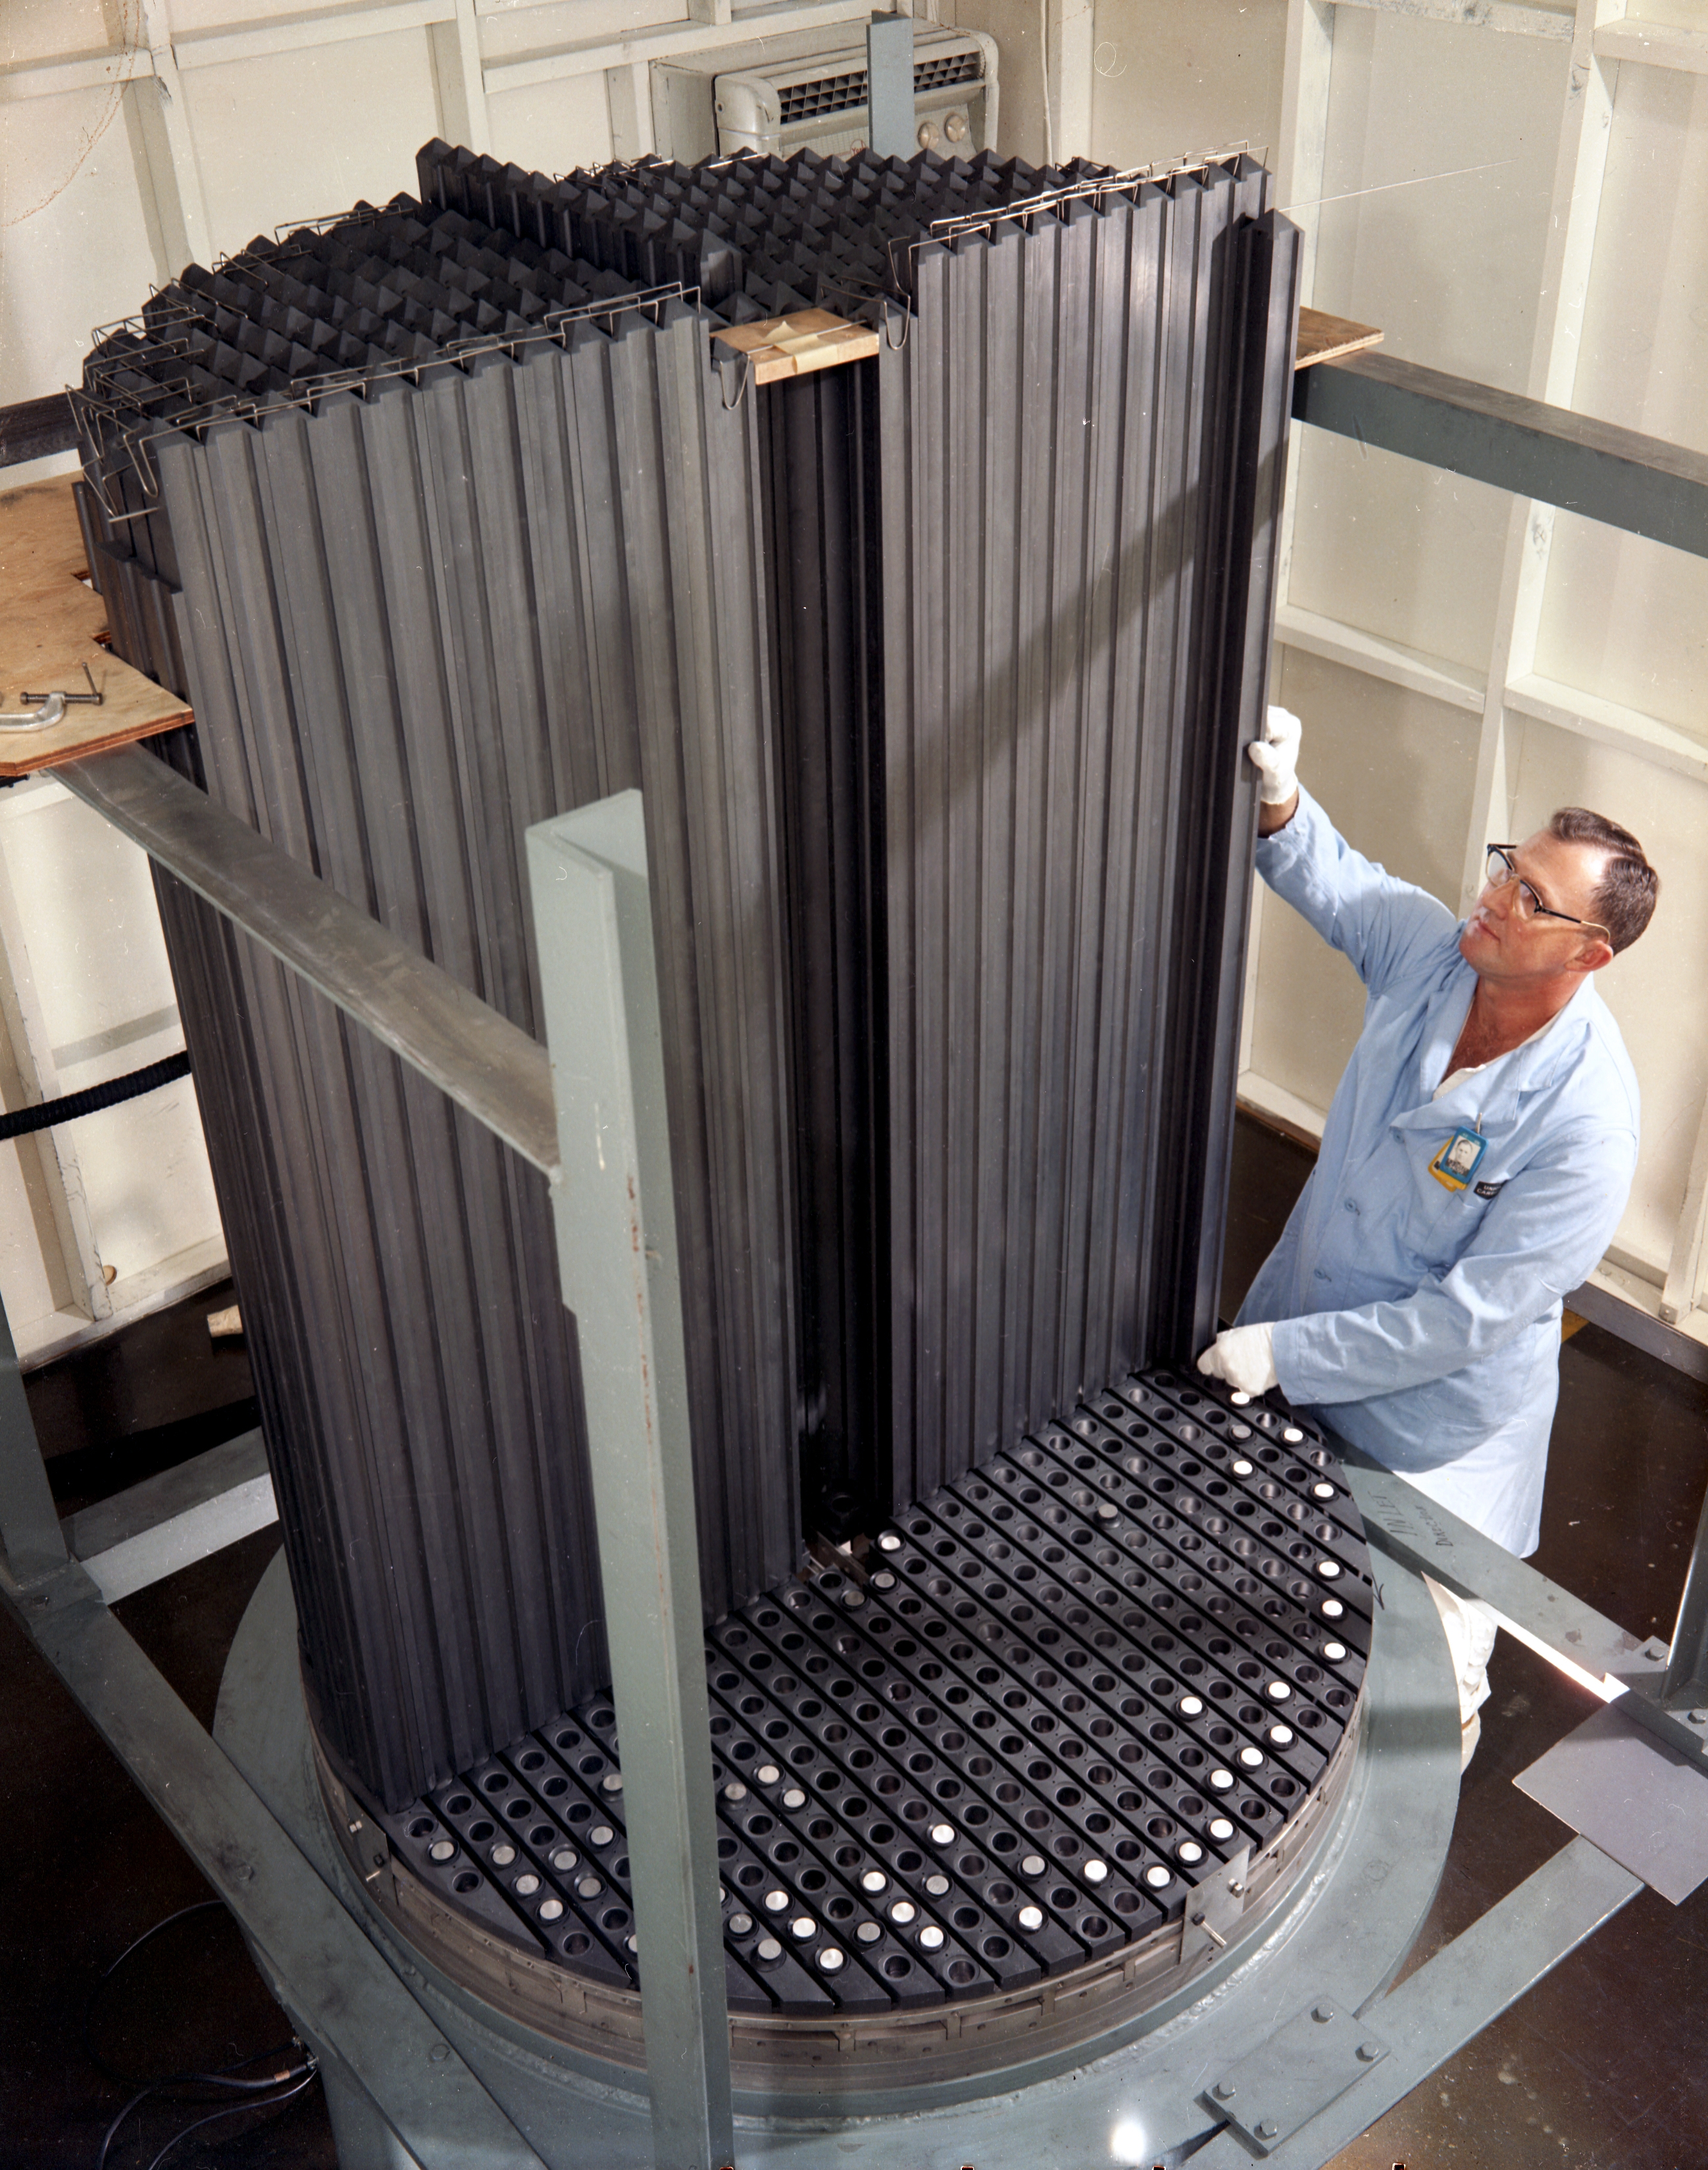
\includegraphics[width=\textwidth]{./images/msre-photo}
      \caption{Graphite assembly for the Molten Salt Reactor Experiment
      \cite{noauthor_measurements_nodate}.}
    \end{figure}
    \column{7cm}
    \begin{table}
      \footnotesize
      \centering
      \caption{Thermal-spectrum MSR designs under active development.}
      \begin{tabular}{l l}
        \toprule
        Reactor & Organization \\
        \midrule
        Integral Molten Salt Reactor & Terrestrial Energy \\
        TMSR-LF & CAS (China) \\
        Compact Molten Salt Reactor & Seaborg Technologies \\
        Copenhagen Atomics Waste Burner & Copenhagen Atomics \\
        \bottomrule
      \end{tabular}
    \end{table}
    \begin{table}
      \footnotesize
      \centering
      \caption{Fast-spectrum MSR designs under active development.}
      \begin{tabular}{l l}
        \toprule
        Reactor & Organization \\
        \midrule
        Molten Chloride Fast Reactor & TerraPower \\
        Molten Salt Fast Reactor & CNRS (France) \\
        Stable Salt Reactor - Wasteburner & Moltex Energy \\
        Molten Chloride Salt Fast Reactor & Elysium Industries \\
        \bottomrule
      \end{tabular}
    \end{table}
  \end{columns}
\end{frame}

\begin{frame}
  \frametitle{Molten Salt Reactor Modeling \& Simulation}
  While modeling MSRs is not necessarily more difficult than modeling solid-fueled reactors, we
  must adapt our software tools to accurately model phenomena unique to MSRs.\\

  \textbf{Phenomena which pose challenges for MSR modeling}
  \begin{itemize}
	\item Strong multiphysics interactions involving neutron flux, temperature, and flow in the
      reactor core
	  \begin{itemize}
		\item Strong temperature feedback due to thermal expansion of liquid fuel salt
		\item Movement of \gls{DNP} along primary coolant loop
        \item Advection-dominated heat transfer as opposed to conduction in solid-fueled reactors
	  \end{itemize}
    \item Loss of delayed neutrons to out-of-core decay
    \item Complex turbulent flow effects in MSRs with wide flow channels
  \end{itemize}
\end{frame}

